\documentclass{article}

\usepackage[margin=2cm]{geometry}
\usepackage{graphicx}
\usepackage{fontspec}

\setmainfont{Segoe UI}
\setmonofont{Fira Code}

\title{Matching Engine}
\author{Billy Sumners}

\begin{document}
\maketitle

\section{Introduction}

The Matching Engine is a tool for creating, cancelling, and matching orders for a hypothetical stock at a hypothetical stock exchange. It provides a REST API to achieve these objectives, as well as querying the system for historial orders and trades.

The system will be based around a SQL database. A Spring Boot application will query this database using JDBC, providing a REST API for a web frontend based on React to talk to. Entities will be validated with Spring/Hibernate. Time permitting, there will be an admin frontend based on Thymeleaf.

\section{Database and Entities}

There are four entities considered in this application, represented as tables in the database and classes in the Java application.

\subsection{Database Entities}

\begin{figure}[h]
    \centering
    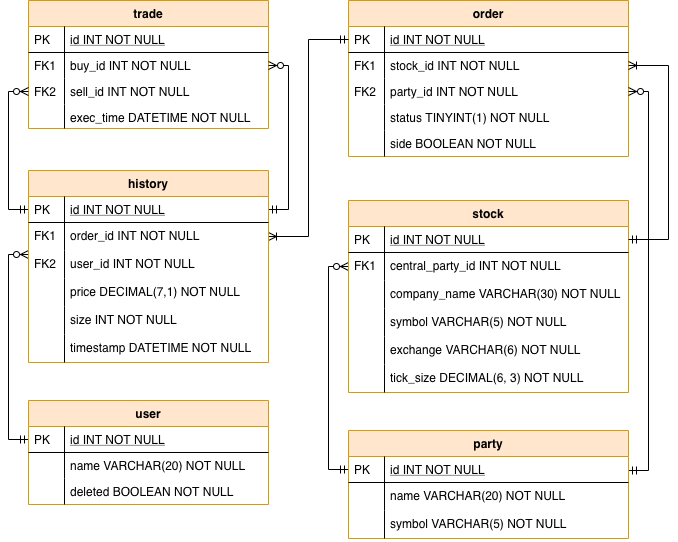
\includegraphics[width=0.7\textwidth]{database-erd.png}
    \caption{Database entity-ralationship diagram}
\end{figure}

\paragraph{Stock} The stock entity corresponds to a stock being traded at the exchange. It has an \texttt{id} to act as the primary key, a \texttt{symbol}, and the \texttt{exchange} the stock is traded at.

\paragraph{Party} The party entity corresponds to an actual party (e.g. a company) trading the stock. It has an \texttt{id} for the primary key, a \texttt{name}, and a \texttt{symbol} to act as an abbreviation of the name.

\paragraph{User} The user entity corresponds to a user working with the application. It has an \texttt{id} to act as the primary key, a \texttt{name} (the username), and a \texttt{deleted} boolean to indicate whether the user is suppressed from the system - deleting the user from the table entirely will break a foreign key constraint with order histories, which we must preserve.

\paragraph{Order} The order entity corresponds to a buy or sell order made in the application. It has an \texttt{id} to act as the primary key, a foreign key \texttt{party\_id} referencing the party owning the stock making the trade, a \texttt{stock\_id} referencing the \texttt{stock} being bought/sold, the \texttt{side} of the order as a boolean (0 = sell, 1 = buy).

\paragraph{History} The \texttt{history} entity corresponds to the history of an order's price and size from when it is first created to when the order is fulfilled or cancelled. It has a \texttt{version\_id} and \texttt{order\_id} to represent the version of a referenced order, acting as the primary key, a \texttt{price}, a \texttt{size}, a \texttt{status} of the order, and a \texttt{timestamp} set to when a \texttt{history} row is made. The idea is that when an order changes its price,  size, or status in the  system  (through user modification or trades being made), a new version is made.

\paragraph{Trade} The trade entity corresponds to a trade made by the application matching a buy order and a sell order. It has an \texttt{id} to act as the primary key, \texttt{buy\_id} and \texttt{sell\_id} referencing the buy and sell order respectively, and an \texttt{execution\_time} when the trade is made.

\subsection{Java Entities}

\begin{figure}[h]
    \centering
    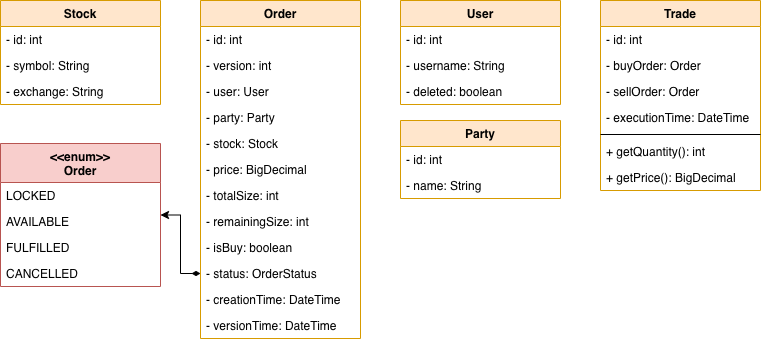
\includegraphics[width=0.7\textwidth]{entities.png}
    \caption{Java entities}
\end{figure}

\paragraph{Stock} The \texttt{Stock} Java class corresponds exactly to the database. A \texttt{Stock} is valid if none of its fields are null, the symbol has length at most 6, and the exchange has length at most 10.

\paragraph{User} The \texttt{User} Java class corresponds exactly to the database, with \texttt{name} being called \texttt{username} in the class A \texttt{User} is valid if none of its fields are null, and its name is at most 20 characters.

\paragraph{Order} The \texttt{Order} class is effectively a combination of the \texttt{order} and \texttt{history} tables. Within the \texttt{Order} class, the \texttt{user\_id} field will be replaced by the referenced user entity, and the \texttt{stock\_id} will be replaced by the referenced stock entity. The boolean field \texttt{isBuy} will take the place of \texttt{side} in the table, being \texttt{true} if the order's side is buy, and \texttt{false} if the side is sell. The reason for this decision is that it will be easier to store in the database. The \texttt{status} field will be an enum matching the \texttt{status} column in the table.

The \texttt{Order} class will take values from the \texttt{history} table for the \texttt{price} and \texttt{remainingSize}. The fields \texttt{creationTime} and \texttt{lotSize} will be the relevant fields taken from the \texttt{history} table for when the order was first created.

An order is valid if none of its fields are null, the price has at most 7 digits with 1 digit after the decimal point, the \texttt{lotSize} and \texttt{remainingSize} is at most 100 000, the status is between 1 and 3, and the creation time is in the past.

\paragraph{Trade} Within Java, the \texttt{buy\_id} and \texttt{sell\_id} will be replaced by the referenced order entities, with the orders set to be as they were at the time of the trade. There will be a \texttt{getQuantity()} property, which will be calculated based on the size of the buy and sell order at the time the trade is made, and a \texttt{getPrice()} property, which will be calculated based on the the price of the sell order at the time the trade is made. 

A trade is valid if none of its fields are null, and the execution time is in the past.

\section{Java Backend}

\begin{figure}[h]
    \centering
    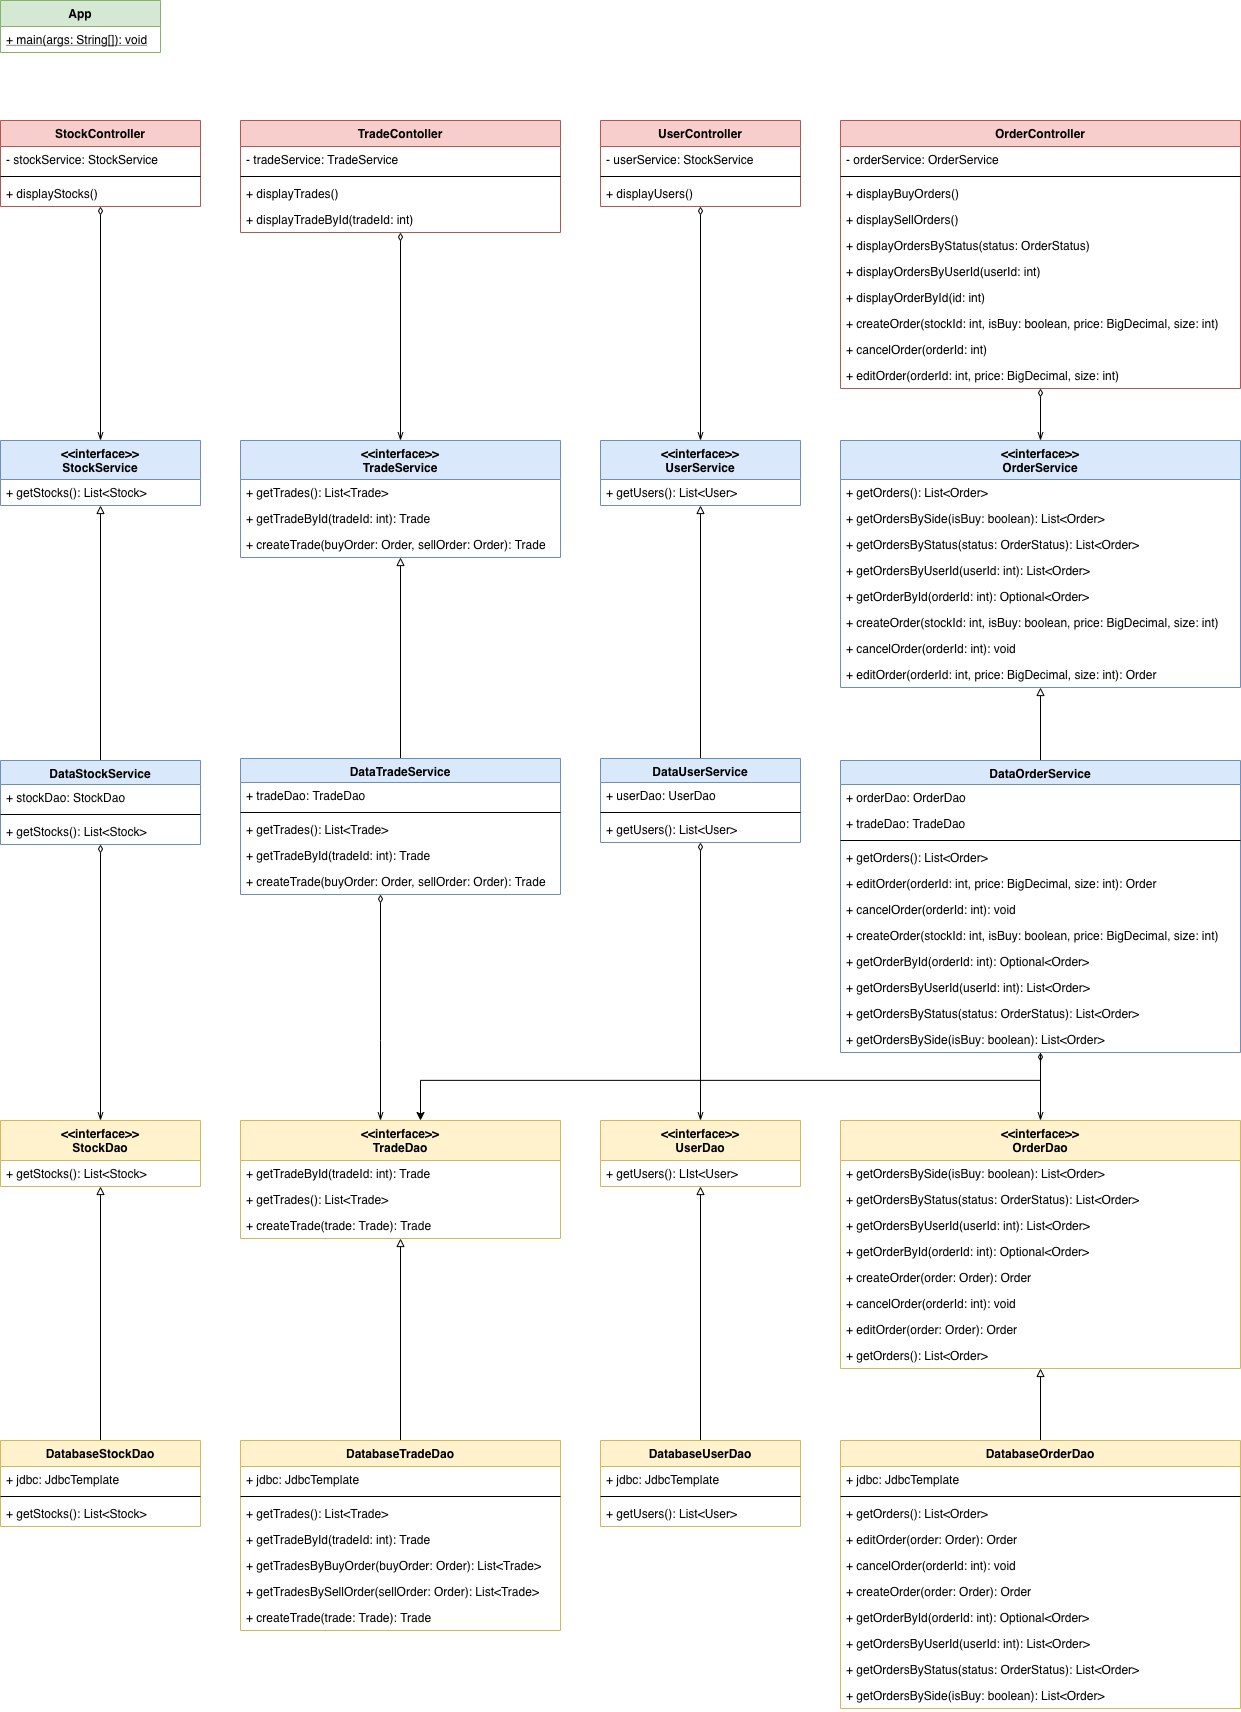
\includegraphics[width=0.9\textwidth]{class-diagram.png}
    \caption{Class diagram}
\end{figure}

Most things in the backend are CRUD. For each Java entity, there is a controller (\texttt{@RestController}), a service layer, and a DAO. The relevant classes for \texttt{Order}s are larger than the others, and most interesting are the \texttt{createOrder(..)} and \texttt{editOrder(..)} methods in the \texttt{OrderService}. These methods take in some preliminary values for a new/edited \texttt{Order}, construct it, check if it's valid (throwing an exception containing a list of validation errors if not), and adds it to the database. It then checks the \texttt{OrderDao} for any matching orders, creating a \texttt{Trade} entity and updating the relevant \texttt{Orders} if so.

\section{REST Endpoints}

\subsection{Stock}

\paragraph{GET /stock} Returns a JSON array of all stocks in the system.

\subsection{Trade}

\paragraph{GET /trade} Returns a JSON array of all trades in the system.

\paragraph{GET /trade/\{id\}} Returns a JSON object of a trade in the system with the given ID if it can be found, and 404 not found otherwise.

\subsection{User}

\paragraph{GET /user} Returns a JSON array of all users in the system.

\subsection{Order}

\paragraph{GET /order/buy} Returns a JSON array of all buy orders in the system.

\paragraph{GET /order/sell} Returns a JSON array of all sell orders in the system.

\paragraph{GET /order/status/\{status\}} Returns a JSON array of all orders with the given status (\texttt{pending}, \texttt{fulfilled}, \texttt{cancelled}). Returns 404 Not Found if the given status does not exist.

\paragraph{\texttt{GET /order/user/\{id\}}} Returns a JSON array of all orders made by the given user, returning 404 Not Found if a user with the given ID does not exist in the system.

\paragraph{\texttt{GET /order/\{id\}}} Returns a JSON object of the order with the given ID, returning 404 Not Found if it cannot be found.

\paragraph{\texttt{POST /order?stock-id=\{stockId\}\&is-buy=\{isBuy\}\&price=\{price\}\&size=\{size\}}} Creates an order in the system with the given parameters, returning a JSON object of the order if it succeeded, and 422 Unprocessable Entity if it did not succeed due to a bad parameter.

\paragraph{\texttt{POST /order/cancel/\{id\}}} Cancels the order with the given ID, returning 404 Not Found if the given order doesn't exist.

\paragraph{\texttt{POST /order/edit/\{id\}?stock-id=\{stockId\}\&is-buy=\{isBuy\}\&price=\{price\}\&size=\{size\}}} Edits an order in the system with the given ID with the given parameters, returning a JSON object of the order if it succeeded, 404 Not Found if the order does not exist, and 422 Unprocessable Entity if it did not succeed due to a bad parameter.

\section{User Frontend}

\end{document}